\section{Introduction}
\label{sec:intro}

This document describes the schematic and functional operation of a 4-channel ADC module prototype, designed in KiCad 9. The module is one building block in a scalable detector-controller system: each board contains its own processor and plugs into a minimal backplane that provides:
\begin{itemize}
  \item A single \SI{12}{\volt} power rail.
  \item A \SI{10}{\mega\hertz} synchronization clock for the DC-DC converters and the detector sequencer
  \item A start signal indicating the beginning of an acquisition cycle.
  \item An emergency-stop line to flag a fault condition.
\end{itemize}
Each board also has its own Gigabit Ethernet port—for configuration, telemetry, and streaming video data

\autoref{fig:pcb_top} and \autoref{fig:pcb_bottom} show the PCB implementation of the 4-channel ADC prototype board with

\begin{multicols}{2}
  \begin{enumerate}
    \item Digital \SI{3.3}{\volt} DC-DC Converter.
    \item Backplane Connector.
    \item Analog \SI{-15.5}{\volt} DC-DC Converter.
    \item RJ45 Ethernet Connector.
    \item Zynq-Soc Module Mode Switch.
    \item Voltage Translator IC.
    \item Analog \SI{5.5}{\volt} DC-DC Converter.
    \item Analog \SI{15.5}{\volt} DC-DC Converter.
    \item FTDI USB-C Interface.
    \item Zynq-Soc Module.
    \item Zynq-Soc Reset Button.
    \item Digital \SI{2.5}{\volt} LDO.
    \item 4 Channel Video Front-End and ADC.
    \item Analog \SI{5}{\volt} LDO.
    \item Analog \SI{2.5}{\volt} LDO.
    \item Analog \SI{4.2}{\volt} LDO.
    \item Analog \SI{15}{\volt} LDO.
    \item Analog \SI{-15}{\volt} LDO.
    \item Video Input Connector.
    \item \SI{12}{\volt} Power Input Protection.
    \item Clock Generator.
    \item EEPROM.
  \end{enumerate}
\end{multicols}

\begin{figure}[!ht]
  \centering
   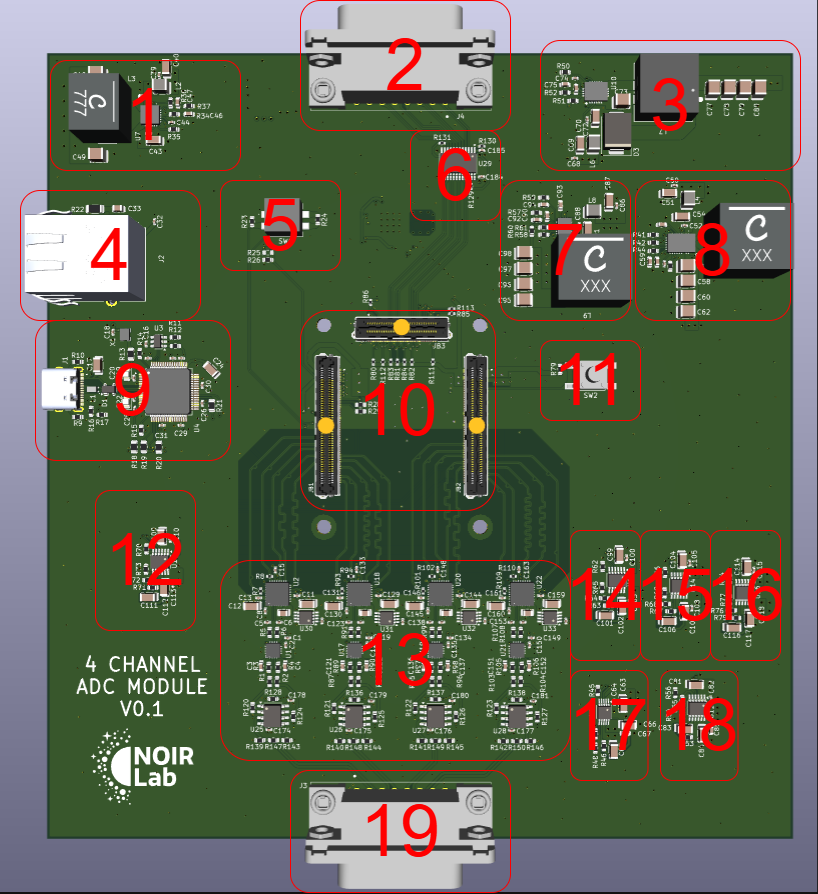
\includegraphics[width=0.8\linewidth]{sections/introduction/top_number.png}
  \caption{Top View of the 16.2 cm x 17.1 cm, six-layer PCB with impedance control, 4-channel ADC prototype board.}
  \label{fig:pcb_top}
\end{figure}

\begin{figure}[!ht]
  \centering
   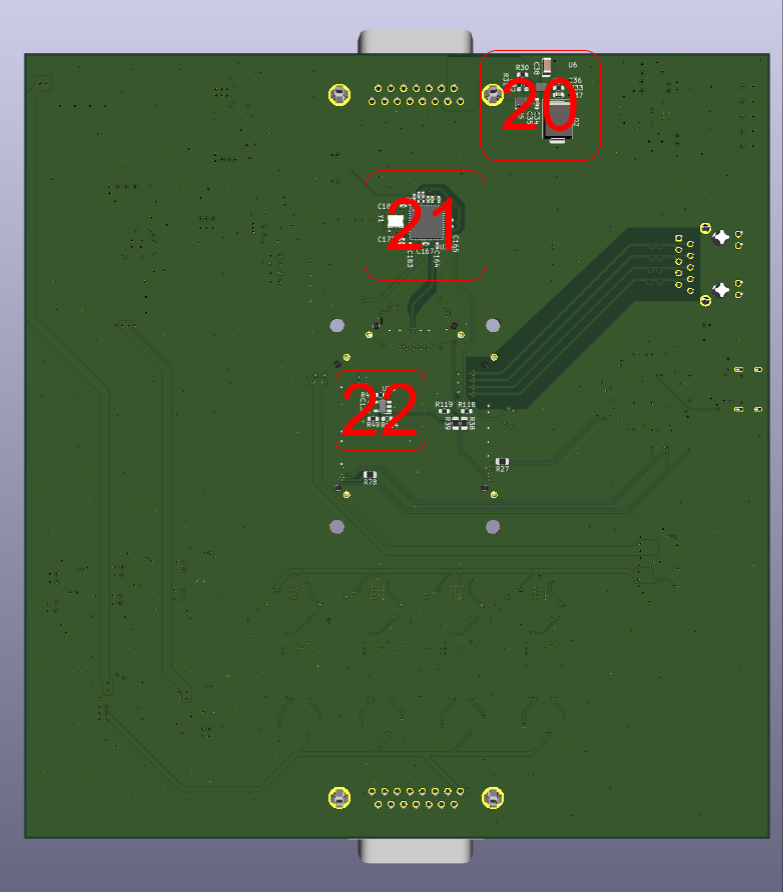
\includegraphics[width=0.8\linewidth]{sections/introduction/bottom_number.png}
  \caption{Bottom View of the 16.2 cm x 17.1 cm, six-layer PCB with impedance control, 4-channel ADC prototype board.}
  \label{fig:pcb_bottom}
\end{figure}

In \autoref{fig:pcb_top}, most of the digital circuitry is clustered on the left side (from top view). Along the top edge you'll find the backplane connector and the DC-DC converters; along the bottom edge are the low-noise LDOs, the four ADC channels with their analog front end, and the input connector.

Immediately beside the top backplane connector, a jitter-attenuator clock generator takes the 10 MHz sync clock from the backplane and delivers a low-jitter reference to the Zynq SoC for the detector sequencer and DC-DC synchronization. A small I²C EEPROM stores the board's type and revision information.

At the center of the board sits a Trenz TE0720-04-62I33MA Zynq SoC-Module, which integrates an AMD Zynq™ 7020-2I, 1 GB of DDR3L RAM, and 8 GB of eMMC flash.

On the left digital side, a Gigabit-Ethernet RJ45 port interfaces with the Zynq SoC for configuration, telemetry, and streaming video data from the ADCs. An FTDI USB-C interface provides direct programming of the Zynq (without a separate JTAG adapter) and supplies a UART console link